\documentclass[a4paper,11pt]{article}

\usepackage{subfigure} 
\usepackage{floatrow}
\usepackage{booktabs}
\usepackage{graphicx}
\usepackage{url}


\begin{document}

\title{Supplementary Information}

\section{Parameter tuning}
We tune the hyper parameters using a 3 fold cross-validation (CV) on the training split. For all baseline regularization parameters %(or a grid search based on the method): 
we tried the range: [$100, 50, 10, 1, 0.1, 0.01, 0.05, 10^{-3}$]. To address the class-skew we 
assign a higher weight to the positives. For BSL-MTL, to tune the rank parameter '$k$' we tried: [1, 5, 10, 25, 40, 60, 100] and the regularization parameter controlling the norm of $U$ and $V$ was tuned over the range $\lambda$=$\{1 ... 10^{-3}\}$. For each task $t$, $\sigma_t$ was varied over the values $[10^{-3}, 10^{-4}, 10^{-5}, 10^{-6}]$ and
$\mu_t$ was varied over $\{0, 0.25, 0.5, 0.75, 1\}$.
The optimal setting was:  $k=10$. %, $\lambda = 0.01$, $\sigma_{ebola}=10^{-5}$, $\sigma_{flu}=\sigma_{hepc}=10^{-6}$.

\section{10 fold cross validation}
In the 10 fold cross-validation (CV) experiments, a much larger training set is available. So the single task baseline becomes much harder to beat as it can independently tune parameters for each task. All methods have a higher variance in their performance (we think this is due to the smaller and hence more variable test data in a 10 fold CV setting). Our method improves on only the \textit{Hep-C} task.

\begin{table*}[h]\caption{Area Under the Precision-Recall curve for 10 fold CV. The first row is the only single-task method and all others are multitask models.}
\label{resultsTable}
\begin{center}
\def\arraystretch{1.2}
\begin{tabular}{c|ccc}
\toprule
& \multicolumn{3}{c}{\textbf{10 fold CV}} \\
& \textit{Ebola} & \textit{Hep-C} & \textit{Influenza} \\ \midrule
 STL     & 0.28$\pm$.11 & 0.74$\pm$.05 & 0.66$\pm$.08  \\ 
 MMTL    & 0.28$\pm$.11 & 0.68$\pm$.04 & 0.40$\pm$.03  \\ 
 Norm    & 0.20$\pm$.09 & 0.70$\pm$.06 & 0.44$\pm$.05  \\ 
 Rank    & 0.18$\pm$.08 & 0.70$\pm$.06 & 0.45$\pm$.04  \\ 
 MTPL    & 0.27$\pm$.08 & 0.67$\pm$.05 & 0.48$\pm$.06  \\ 
 IMC     & 0.16$\pm$.08 & 0.72$\pm$.06 & 0.45$\pm$.06  \\ 
 BSL-MTL & 0.28$\pm$.11 & 0.82$\pm$.05 & 0.62$\pm$.02  \\ 
\bottomrule
\end{tabular}
\end{center}
\end{table*}

%%%%%%%%%%%%%%%%%%%%%%%%%%%%%%%%%

\section{Homologous interactions}
Since we use data from several strains for each task, the PPI data contains some interactions that are interologs.
We observed this for two of the tasks: \textit{Hepatitis-C} and \textit{Influenza A}. Note that we did not find any interologs \textit{across} tasks. These homologous interactions in the various strains are reported by different experimental studies and we believe their presence suggests the confidence of such interactions. Since we use only PPI derived from experimental methods (and not electronically inferred), we do not exclude any homologous interactions from our training. \\
\textbf{Removing homologs from the evaluation}:\\
\noindent The number of distinct PPI for which interologs or homologs exist is very small ($\approx$20), but there are several homologs for each such PPI. Note that any benefits achieved from the presence of homologous interactions will be available to all the methods (since the models were built using identical train/test data). Here we present results on the 10\% setting by removing all homologs from the test data (note: the \textit{Ebola} task did not have any homologs). For lack of space we only mention the trend for our method (BSL-MTL) - \textit{Hep-C}: 0.85 and \textit{Influenza:} 0.45. The other methods show a similar trend; our method continues to outperform by significant margins.


\section{Biological significance of interactions} 
 \noindent\emph{Phosphorylation sites}: 
 We found the frequent occurrence of S and T and sometimes Y in the motifs striking and suspected this may be
 related to the amino acids being frequent targets of phosphorylation.
 Phosphorylated sites often serve as PPI sites, and databases such as Phosphosite \cite{phosphosite} are
  repositories for known sites in human proteins. Since these are sites in human proteins, we searched for the patterns
	from the 4-mer motif in Fig \ref{fig:human_motifs} and found several to be flanking known phosphorylation sites in human proteins:
	\texttt{LLLs}, \texttt{LLLt}, \texttt{ILLs}, \texttt{PPPs}, \texttt{PIPs}, \texttt{PIPt}, \texttt{LIPs}, \texttt{PLLt} (lower-case indicates the putative phosphorylation site). This observation also supports the notion that the motifs predictive
	of interaction are biologically significant.

\noindent\emph{Evidence in IEDB}\footnote{\url{www.iedb.org}}:
We found experimental evidence for the significance for the virus motifs in the Immune Epitope\footnote{An epitope is a very short sequence from the virus that binds to human antibodies} database (IEDB) \cite{iedb}.
The pattern \texttt{IVGG} from the \textit{Hepatitis-C} motif in Fig. \ref{fig:hepc_motifs} is found in 53 epitopes.
From the \textit{Ebola} motifs in Fig \ref{fig:ebola_motifs}, we find that \texttt{TLAT} is part of six different epitopes, \texttt{SLTT} appears in three epitopes. \texttt{PLIK}, \texttt{SLLL} from the \textit{Influenza} motif are also found in many epitopes.
Finding that the virus k-mer patterns predicted by our method are recognized by human antibodies
is a further validation of its performance.
Further, using higher dimensional $k$-mers (where $k$=7, 8, 9) as
features in our model will give motifs from which complete epitopes can be derived. % which can then be verified by biochemical peptide interaction assays.
Our model thus has applications in epitope prediction as well, where conventional methods consist of scanning all possible $k$-mers from protein sequences to identify likely epitopes.



\begin{figure}[h]
\begin{floatrow}
\ffigbox[0.4\columnwidth]{%
%trim option's parameter order: left bottom right top
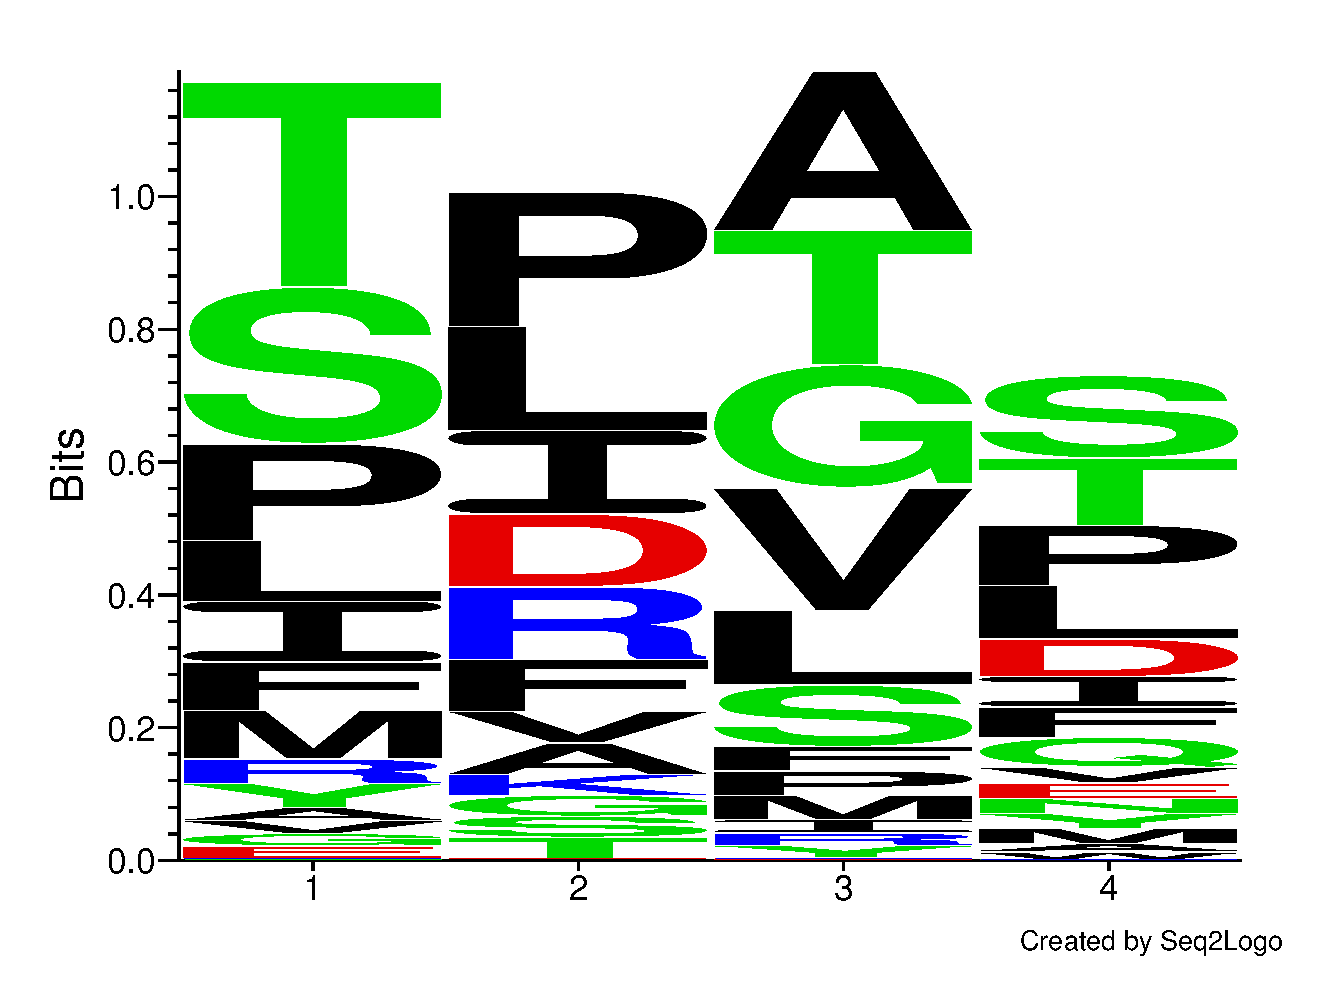
\includegraphics[scale=0.25, trim = 0.2cm 0 0 0]{fig7-eps-converted-to.pdf}
}{%
\caption{Sequence motif from top four-mer features specific to \textit{Ebola} proteins}%
\label{fig:ebola_motifs}
}

\ffigbox[0.4\columnwidth]{%
%trim option's parameter order: left bottom right top
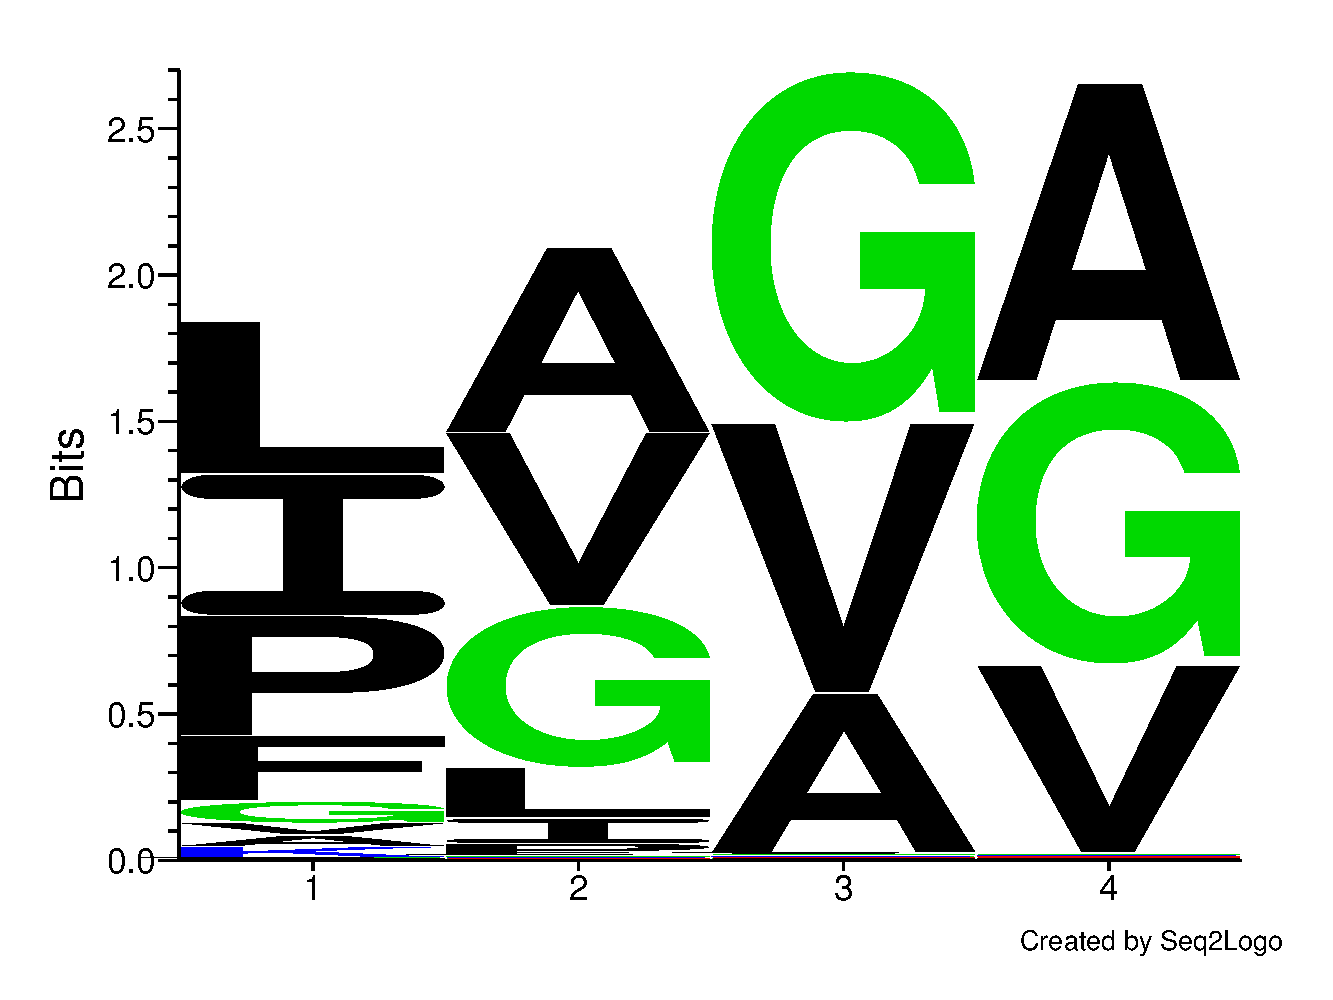
\includegraphics[scale=0.25, trim = 0 0 0 0]{fig8-eps-converted-to.pdf}
}{%
\caption{Sequence motifs specific to \textit{Hepatitic-C} proteins that are also important to interactions.}%
\label{fig:hepc_motifs}
}


\end{floatrow}
\end{figure}

\begin{figure}[h]
\begin{floatrow}
\ffigbox[0.4\columnwidth]{%
%trim option's parameter order: left bottom right top
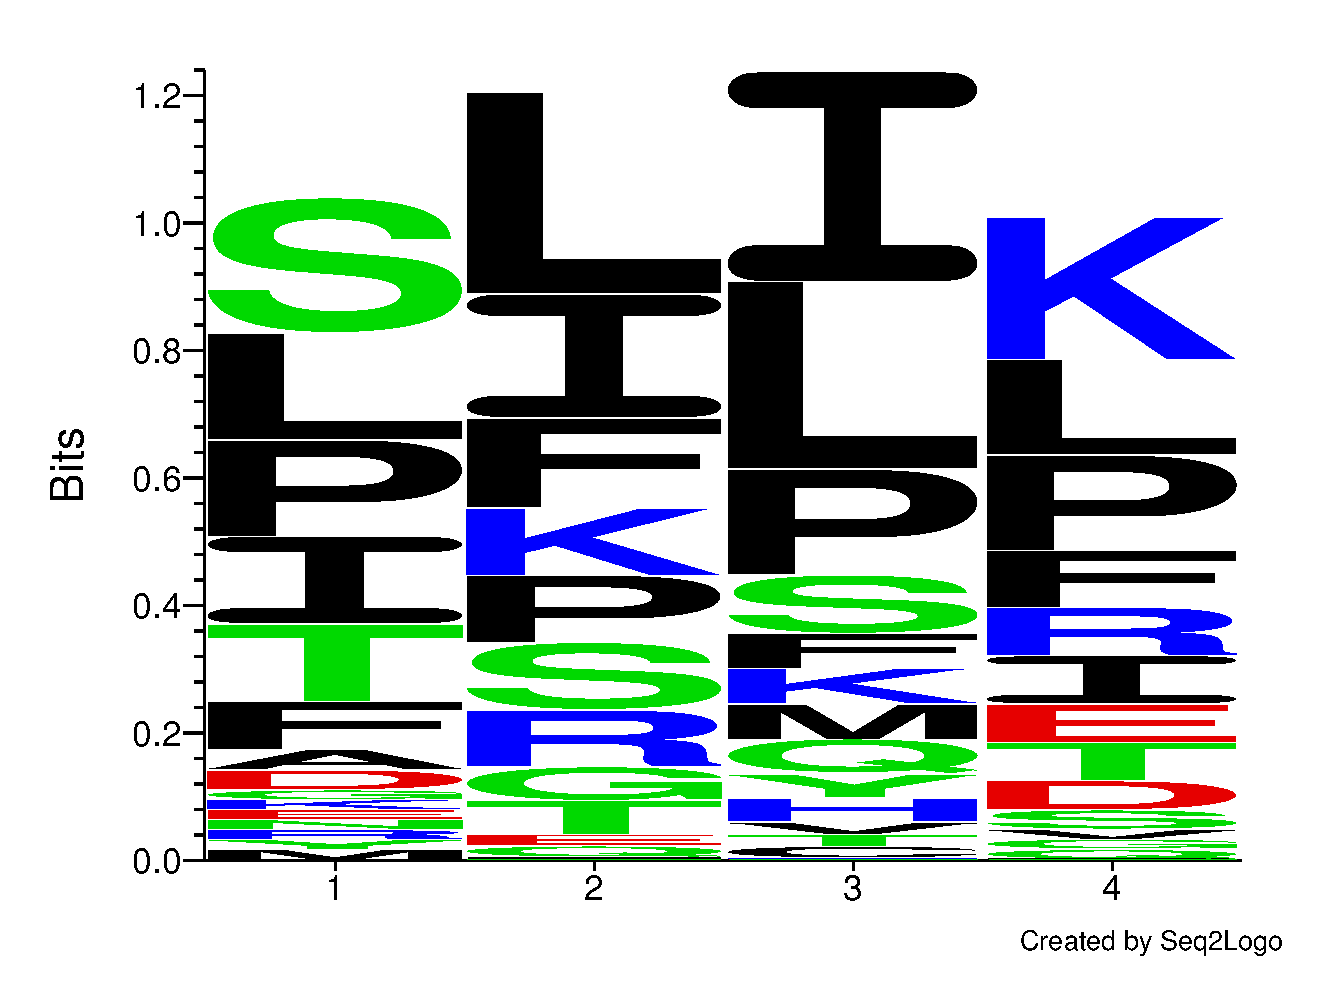
\includegraphics[scale=0.25, trim = 0 0 0 0]{fig9-eps-converted-to.pdf}
}{%
\caption{Sequence motifs specific to \textit{Influenza} proteins that are also important to interactions.}%
\label{fig:flu_motifs}
}
\end{floatrow}
\end{figure}

\newpage

\section{Tri-mers}

Below, we show the sequence motifs from the tri-mers found to be highly relevant to predicting interactions between human and viral proteins.

\begin{figure}[h]
\begin{floatrow}
\ffigbox[0.4\columnwidth]{%
%trim option's parameter order: left bottom right top
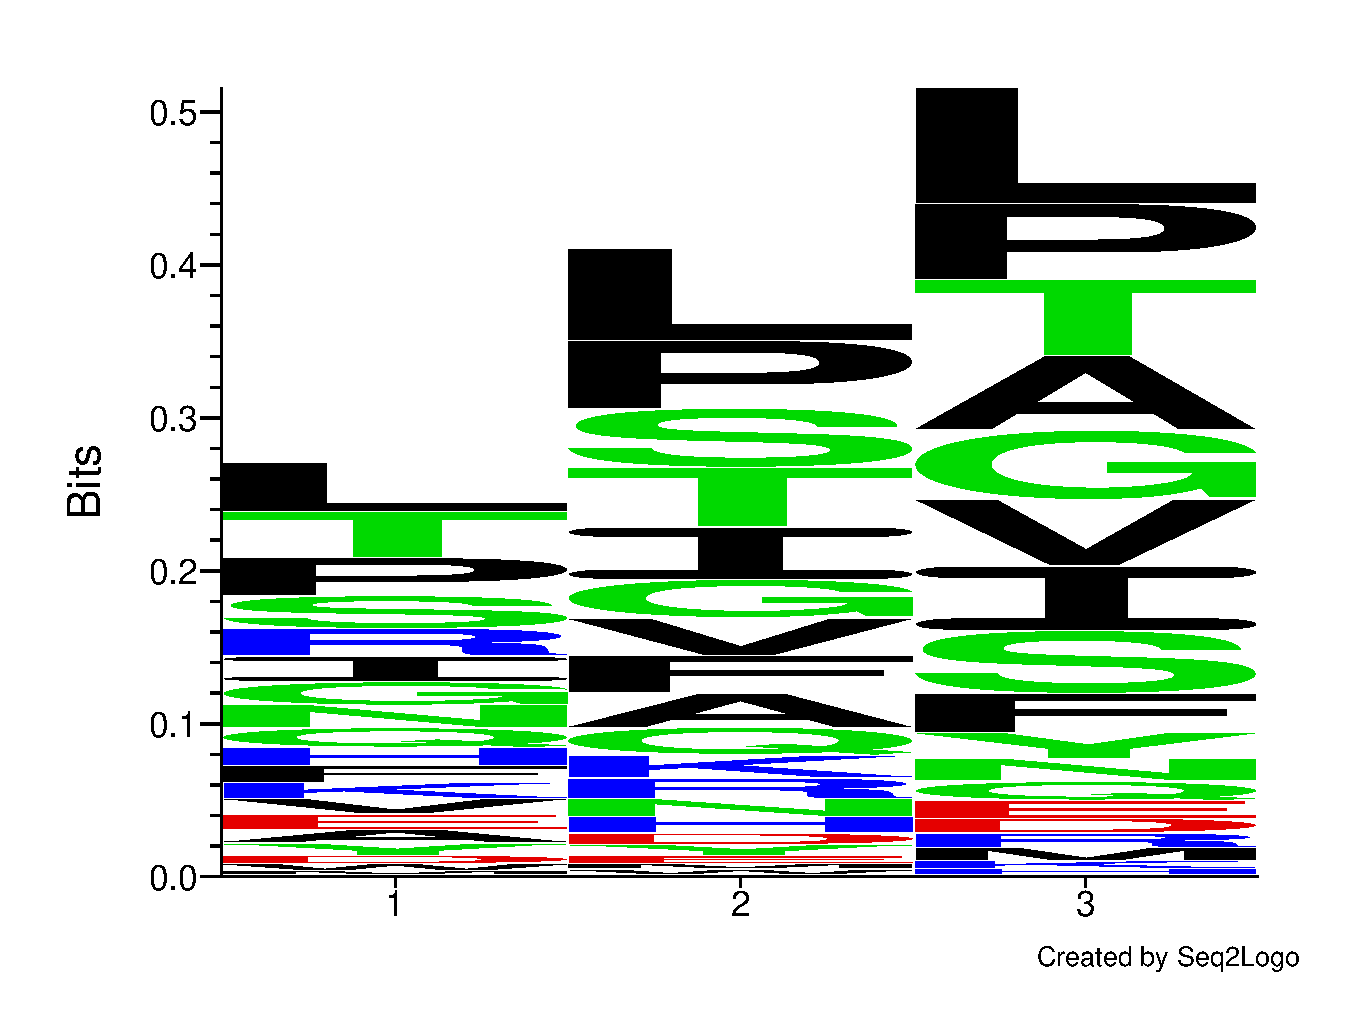
\includegraphics[scale=0.25, trim = 0 0 0 0]{top10ebola_3mers_seq2logo.eps}
}{%
\caption{Sequence motifs specific to \textit{Ebola} proteins that are also important to interactions.}%
\label{fig:hepc_motifs}
}

\ffigbox[0.4\columnwidth]{%
%trim option's parameter order: left bottom right top
\includegraphics[scale=0.25, trim = 0 0 0 0]{top10flavi_3mers_seq2logo.eps}
}{%
\caption{Sequence motifs specific to \textit{Hepatitic-C} proteins that are also important to interactions.}%
\label{fig:hepc_motifs}
}
\end{floatrow}
\end{figure}

\begin{figure}[h]
\begin{floatrow}
\ffigbox[0.4\columnwidth]{%
%trim option's parameter order: left bottom right top
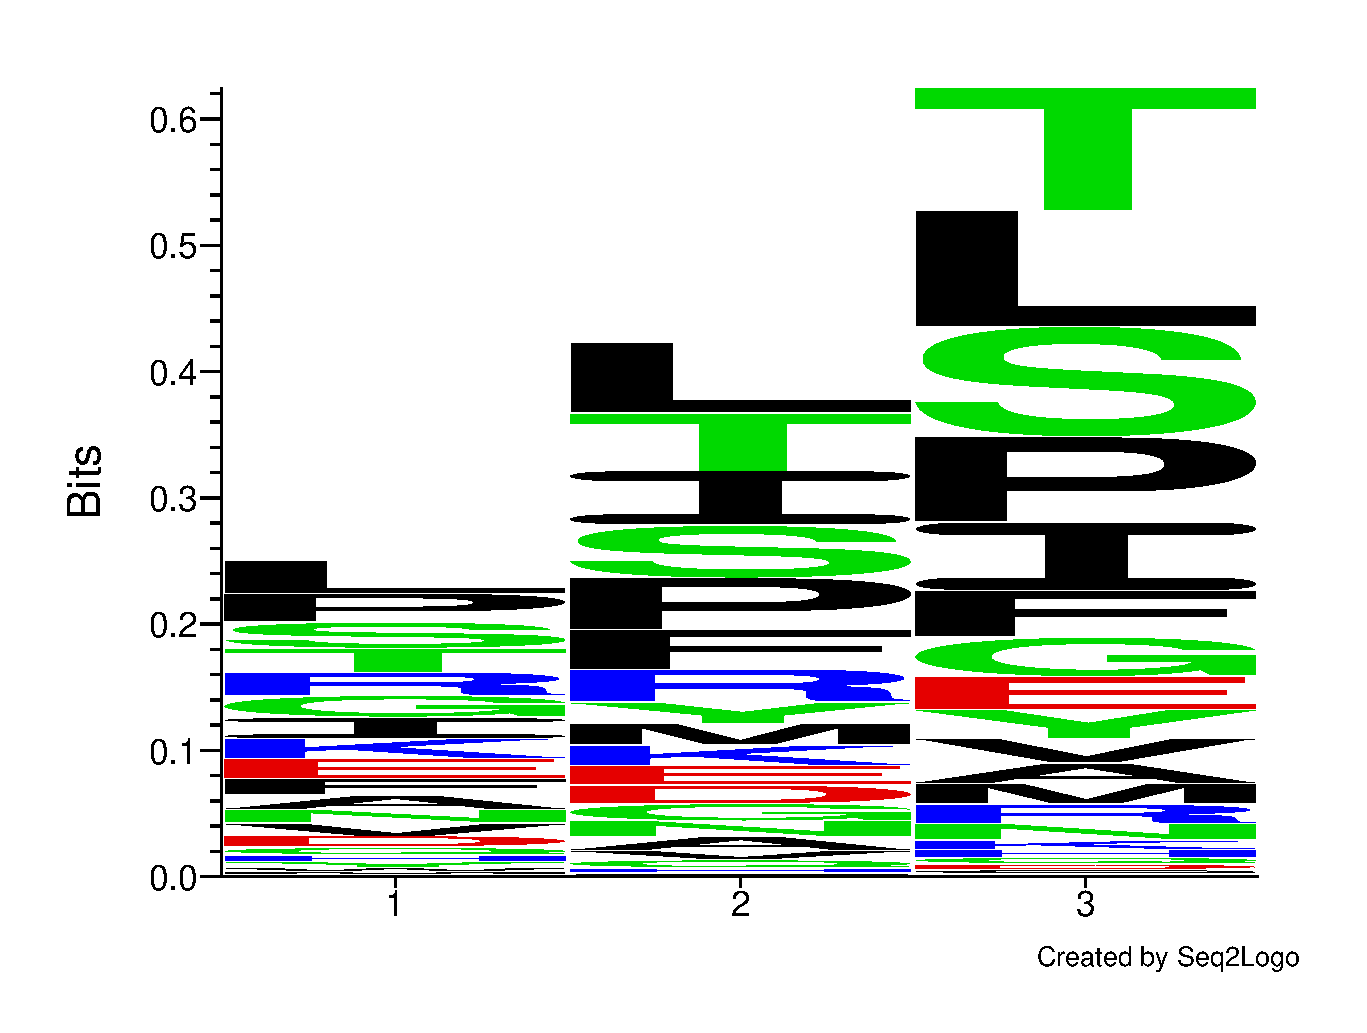
\includegraphics[scale=0.25, trim = 0 0 0 0]{top10flu_3mers_seq2logo.eps}
}{%
\caption{Sequence motifs specific to \textit{Influenza} proteins that are also important to interactions.}%
\label{fig:flu_motifs}
}
\ffigbox[0.4\columnwidth]{%
%trim option's parameter order: left bottom right top
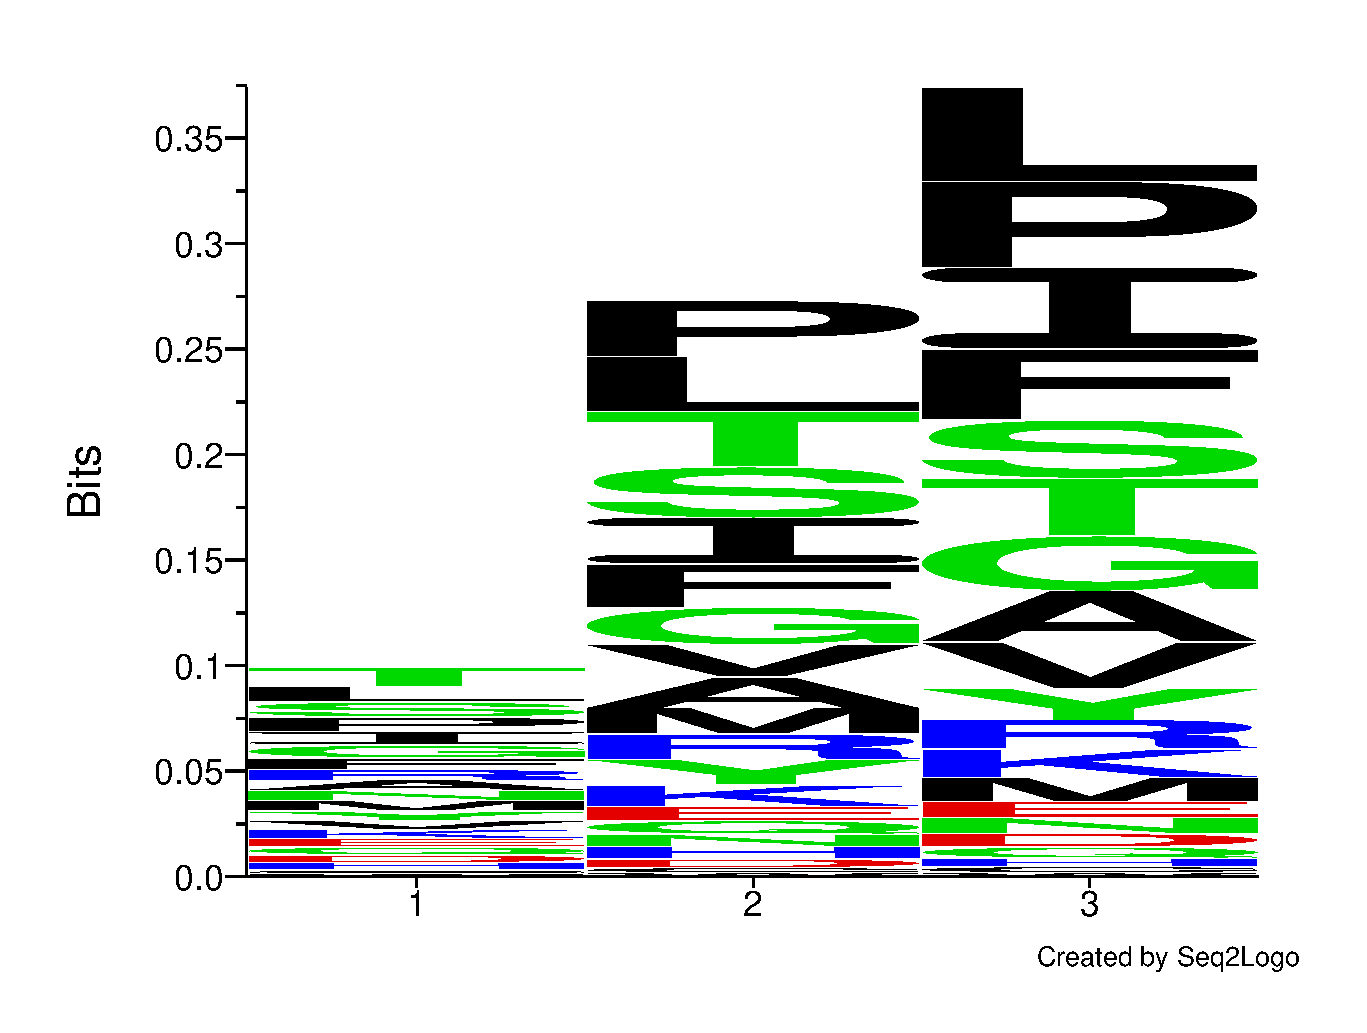
\includegraphics[scale=0.25, trim = 0 0 0 0]{top20human_3mers_seq2logo.eps}
}{%
\caption{Sequence motif constructed from the top tri-mer features of human proteins}%
\label{fig:human_motifs}
}
\end{floatrow}
\end{figure}

\bibliographystyle{plain}
\bibliography{references}

\end{document}
